% Chapter 4

\chapter{Results} % Main chapter title

\label{Chapter4} % For referencing the chapter elsewhere, use \ref{Chapter1} 
This section presents the results from implementing the operation described in chapter 4.

% \section{Generation of synthetic plant leaf Images}
For the experiment, every image in the 513 diseased leaf collection was overlaid on the 463 sugar beet images. As a result of the experiment, 237 520 synthetic images were created. Figure \ref{fig:my_gen_6} and \ref{fig:my_gen_7} are random images from the generated dataset.

\begin{figure}[!htb]
    \centering
    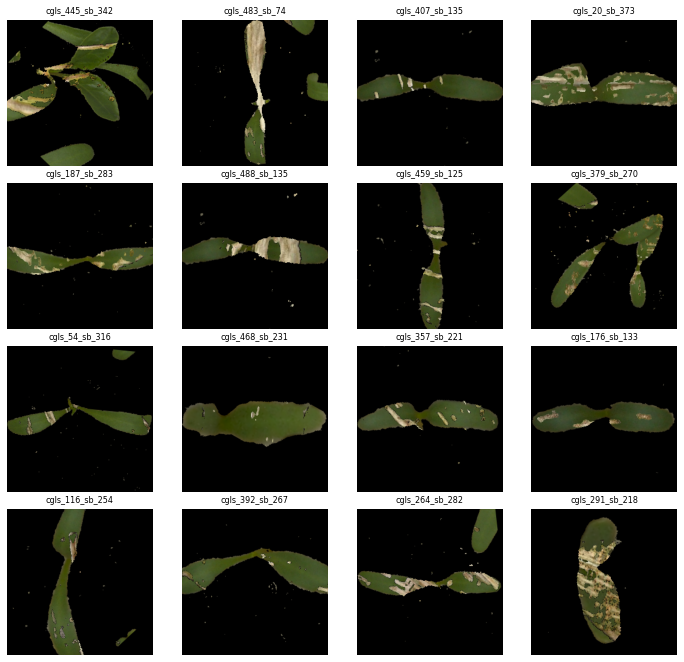
\includegraphics[scale=0.68, keepaspectratio]{Template/Figures/notebook/gen-11.png}
    \caption{Sample image from the image folder}
    \label{fig:my_gen_6}
\end{figure} 

\begin{figure}[!htb]
    \centering
    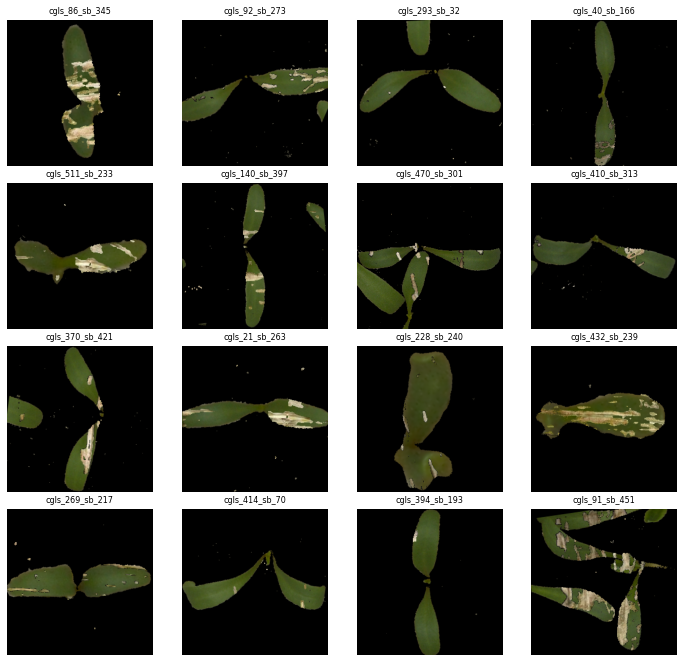
\includegraphics[scale=0.68, keepaspectratio]{Template/Figures/notebook/gen-12.png}
    \caption{Sample image from the image folder}
    \label{fig:my_gen_7}
\end{figure} 